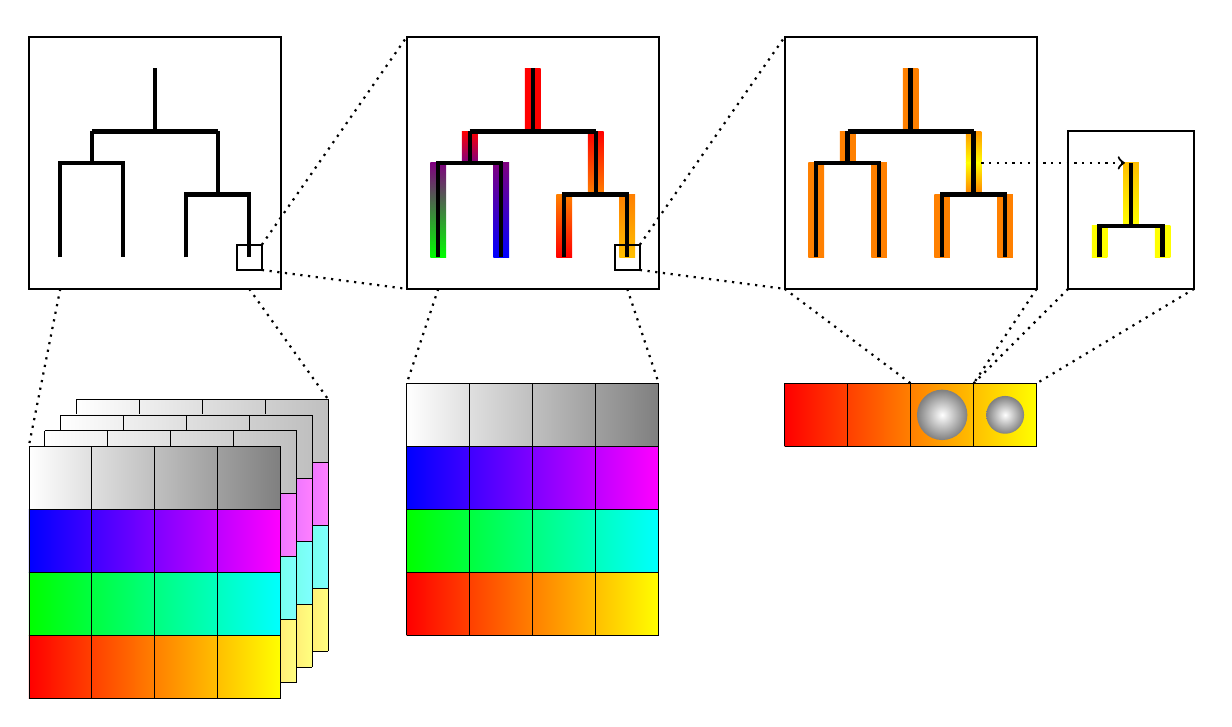
\begin{tikzpicture} [thick, scale=0.8,rotate=0]
  % Shade underneath left phylogeny
  % \shade[top color=red!100!yellow,bottom color=red!100!yellow] (0.5-0.124,6.0) rectangle (0.5+0.124,5.0);
  % \shade[top color=red!100!yellow,bottom color=red!50!blue] (-0.5-0.124,5.0) rectangle (-0.5+0.124,4.5);
  % \shade[top color=red!100!yellow,bottom color=red!50!yellow] ( 1.5-0.124,5.0) rectangle ( 1.5+0.124,4.0);

  % \shade[top color=red!50!blue,bottom color=red!0!green] (-1.0-0.124,4.5) rectangle (-1.0+0.124,3.0);
  % \shade[top color=red!50!blue,bottom color=blue!100!purple] ( 0.0-0.124,4.5) rectangle ( 0.0+0.124,3.0);
  % \shade[top color=red!50!yellow,bottom color=red!100!yellow] ( 1.0-0.124,4.0) rectangle ( 1.0+0.124,3.0);
  % \shade[top color=red!50!yellow,bottom color=red!25!yellow] ( 2.0-0.124,4.0) rectangle ( 2.0+0.124,3.0);
  % Left species phylogeny
  \draw[] (-1.5,2.5) rectangle (2.5,6.5); 
  \draw[ultra thick] ( 0.5,6.0) node {} -- ( 0.5,5.0) node {}; 
  \draw[ultra thick] (-0.5,5.0) node {} -- ( 1.5,5.0) node {}; 
  \draw[ultra thick] (-0.5,5.0) node {} -- (-0.5,4.5) node {}; 
  \draw[ultra thick] ( 1.5,5.0) node {} -- ( 1.5,4.0) node {}; 
  \draw[ultra thick] (-1.0,3.0) node {} -- (-1.0,4.5) node {} -- ( 0.0,4.5) node {} -- ( 0.0,3.0) node {}; 
  \draw[ultra thick] ( 1.0,3.0) node {} -- ( 1.0,4.0) node {} -- ( 2.0,4.0) node {} -- ( 2.0,3.0) node {}; 

  % Shade underneath middle phylogeny
  \shade[shift={(6 cm,0 cm)},top color=red!100!yellow,bottom color=red!100!yellow] (0.5-0.124,6.0) rectangle (0.5+0.124,5.0);
  \shade[shift={(6 cm,0 cm)},top color=red!100!yellow,bottom color=red!50!blue] (-0.5-0.124,5.0) rectangle (-0.5+0.124,4.5);
  \shade[shift={(6 cm,0 cm)},top color=red!100!yellow,bottom color=red!50!yellow] ( 1.5-0.124,5.0) rectangle ( 1.5+0.124,4.0);

  \shade[shift={(6 cm,0 cm)},top color=red!50!blue,bottom color=red!0!green] (-1.0-0.124,4.5) rectangle (-1.0+0.124,3.0);
  \shade[shift={(6 cm,0 cm)},top color=red!50!blue,bottom color=blue!100!purple] ( 0.0-0.124,4.5) rectangle ( 0.0+0.124,3.0);
  \shade[shift={(6 cm,0 cm)},top color=red!50!yellow,bottom color=red!100!yellow] ( 1.0-0.124,4.0) rectangle ( 1.0+0.124,3.0);
  \shade[shift={(6 cm,0 cm)},top color=red!50!yellow,bottom color=red!25!yellow] ( 2.0-0.124,4.0) rectangle ( 2.0+0.124,3.0);
  % Middle species phylogeny
  \draw[shift={(6 cm,0 cm)}] (-1.5,2.5) rectangle (2.5,6.5); 
  \draw[shift={(6 cm,0 cm)},ultra thick] ( 0.5,6.0) node {} -- ( 0.5,5.0) node {}; 
  \draw[shift={(6 cm,0 cm)},ultra thick] (-0.5,5.0) node {} -- ( 1.5,5.0) node {}; 
  \draw[shift={(6 cm,0 cm)},ultra thick] (-0.5,5.0) node {} -- (-0.5,4.5) node {}; 
  \draw[shift={(6 cm,0 cm)},ultra thick] ( 1.5,5.0) node {} -- ( 1.5,4.0) node {}; 
  \draw[shift={(6 cm,0 cm)},ultra thick] (-1.0,3.0) node {} -- (-1.0,4.5) node {} -- ( 0.0,4.5) node {} -- ( 0.0,3.0) node {}; 
  \draw[shift={(6 cm,0 cm)},ultra thick] ( 1.0,3.0) node {} -- ( 1.0,4.0) node {} -- ( 2.0,4.0) node {} -- ( 2.0,3.0) node {}; 
  % Zoomer between left and middle
  \draw[] (2.0-0.2,3.0-0.2) rectangle (2.0+0.2,3.0+0.2); 
  \draw[dotted] (2.0+0.2,3.0+0.2) node {} -- (4.5,6.5) node {}; 
  \draw[dotted] (2.0+0.2,3.0-0.2) node {} -- (4.5,2.5) node {}; 


  
  
  %  
  % THIRD PHYLOGENY  
  %
  % Shade underneath third phylogeny
  \shade[shift={(12 cm,0 cm)},top color=red!50!yellow,bottom color=red!50!yellow] (0.5-0.124,6.0) rectangle (0.5+0.124,5.0);
  \shade[shift={(12 cm,0 cm)},top color=red!50!yellow,bottom color=red!50!yellow] (-0.5-0.124,5.0) rectangle (-0.5+0.124,4.5);
  \shade[shift={(12 cm,0 cm)},top color=red!40!yellow,bottom color=red!1!yellow] ( 1.5-0.124,5.0) rectangle ( 1.5+0.124,4.5); % Colonization
  \shade[shift={(12 cm,0 cm)},top color=red!1!yellow,bottom color=red!50!yellow] ( 1.5-0.124,4.5) rectangle ( 1.5+0.124,4.0); % Colonization, -10 to emphasisze
  \shade[shift={(12 cm,0 cm)},top color=red!50!yellow,bottom color=red!50!yellow] (-1.0-0.124,4.5) rectangle (-1.0+0.124,3.0);
  \shade[shift={(12 cm,0 cm)},top color=red!50!yellow,bottom color=red!50!yellow] ( 0.0-0.124,4.5) rectangle ( 0.0+0.124,3.0);
  \shade[shift={(12 cm,0 cm)},top color=red!50!yellow,bottom color=red!50!yellow] ( 1.0-0.124,4.0) rectangle ( 1.0+0.124,3.0);
  \shade[shift={(12 cm,0 cm)},top color=red!50!yellow,bottom color=red!50!yellow] ( 2.0-0.124,4.0) rectangle ( 2.0+0.124,3.0);
  % Fourth species phylogeny
  \draw[shift={(12 cm,0 cm)}] (-1.5,2.5) rectangle (2.5,6.5); 
  \draw[shift={(12 cm,0 cm)},ultra thick] ( 0.5,6.0) node {} -- ( 0.5,5.0) node {}; 
  \draw[shift={(12 cm,0 cm)},ultra thick] (-0.5,5.0) node {} -- ( 1.5,5.0) node {}; 
  \draw[shift={(12 cm,0 cm)},ultra thick] (-0.5,5.0) node {} -- (-0.5,4.5) node {}; 
  \draw[shift={(12 cm,0 cm)},ultra thick] ( 1.5,5.0) node {} -- ( 1.5,4.0) node {}; 
  \draw[shift={(12 cm,0 cm)},ultra thick] (-1.0,3.0) node {} -- (-1.0,4.5) node {} -- ( 0.0,4.5) node {} -- ( 0.0,3.0) node {}; 
  \draw[shift={(12 cm,0 cm)},ultra thick] ( 1.0,3.0) node {} -- ( 1.0,4.0) node {} -- ( 2.0,4.0) node {} -- ( 2.0,3.0) node {}; 
  % Shade underneath third phylogeny
  \shade[shift={(12 cm,0 cm)},top color=red!25!yellow,bottom color=red!00!yellow]  (4.0-0.124,4.5) rectangle (4.0+0.124,3.5);
  \shade[shift={(12 cm,0 cm)},top color=red!00!yellow,bottom color=red!00!yellow]  (3.5-0.124,3.5) rectangle (3.5+0.124,3.0);
  \shade[shift={(12 cm,0 cm)},top color=red!00!yellow,bottom color=red!00!yellow]  (4.5-0.124,3.5) rectangle (4.5+0.124,3.0);
  % Fourth species phylogeny
  \draw[shift={(12 cm,0 cm)},] ( 3.0,2.5) rectangle (5.0,5.0); 
  \draw[shift={(12 cm,0 cm)},ultra thick] ( 4.0,4.5) node {} -- ( 4.0,3.5) node {}; 
  \draw[shift={(12 cm,0 cm)},ultra thick] ( 3.5,3.0) node {} -- ( 3.5,3.5) node {} -- ( 4.5,3.5) node {} -- ( 4.5,3.0) node {}; 
  % Colonization line
  \draw[shift={(12 cm,0 cm)},dotted,->] ( 1.5,4.5) node {} -- (4.0-0.1,4.5) node {}; 
  
  
  
  
  
  
  
  
  
  
  
  
  
  
  
  
  
  
  
  
  
  % Zoomer between middle and right
  \draw[shift={(6 cm,0 cm)}] (2.0-0.2,3.0-0.2) rectangle (2.0+0.2,3.0+0.2); 
  \draw[shift={(6 cm,0 cm)},dotted] (2.0+0.2,3.0+0.2) node {} -- (4.5,6.5) node {}; 
  \draw[shift={(6 cm,0 cm)},dotted] (2.0+0.2,3.0-0.2) node {} -- (4.5,2.5) node {}; 

  % Species of left phylogeny
  % BACKGROUND 1
  % Patch gradients
  \shade[shift={(-0.75 cm,-3.25 cm)},left color=red,right color=yellow!50!white] (0,0) rectangle (4,1);
  \shade[shift={(-0.75 cm,-3.25 cm)},left color=green,right color=cyan!50!white] (0,1) rectangle (4,2);
  \shade[shift={(-0.75 cm,-3.25 cm)},left color=blue,right color=magenta!50!white] (0,2) rectangle (4,3);
  \shade[shift={(-0.75 cm,-3.25 cm)},left color=white,right color=gray!50!white] (0,3) rectangle (4,4);
  % Species gradients
  % \shade[shift={(-0.75 cm,-3.25 cm)},inner color=white,outer color=gray] (2.5,3.5) circle (0.4 cm);
  % Grids
  \draw[shift={(-0.75 cm,-3.25 cm)},step=1cm,black,very thin] (0,0) grid ( 4,4); 
  % BACKGROUND 2
  % Patch gradients
  \shade[shift={(-1.0 cm,-3.5 cm)},left color=red,right color=yellow!50!white] (0,0) rectangle (4,1);
  \shade[shift={(-1.0 cm,-3.5 cm)},left color=green,right color=cyan!50!white] (0,1) rectangle (4,2);
  \shade[shift={(-1.0 cm,-3.5 cm)},left color=blue,right color=magenta!50!white] (0,2) rectangle (4,3);
  \shade[shift={(-1.0 cm,-3.5 cm)},left color=white,right color=gray!50!white] (0,3) rectangle (4,4);
  % Species gradients
  % \shade[shift={(-1.0 cm,-3 cm)},inner color=white,outer color=gray] (2.5,3.5) circle (0.4 cm);
  % Grids
  \draw[shift={(-1.0 cm,-3.5 cm)},step=1cm,black,very thin] (0,0) grid ( 4,4); 
  % BACKGROUND 3
  % Patch gradients
  \shade[shift={(-1.25 cm,-3.75 cm)},left color=red,right color=yellow!50!white] (0,0) rectangle (4,1);
  \shade[shift={(-1.25 cm,-3.75 cm)},left color=green,right color=cyan!50!white] (0,1) rectangle (4,2);
  \shade[shift={(-1.25 cm,-3.75 cm)},left color=blue,right color=magenta!50!white] (0,2) rectangle (4,3);
  \shade[shift={(-1.25 cm,-3.75 cm)},left color=white,right color=gray!50!white] (0,3) rectangle (4,4);
  % Species gradients
  % \shade[shift={(-1.0 cm,-3 cm)},inner color=white,outer color=gray] (2.5,3.5) circle (0.4 cm);
  % Grids
  \draw[shift={(-1.25 cm,-3.75 cm)},step=1cm,black,very thin] (0,0) grid ( 4,4); 
  % FOREGROUND
  % Patch gradients
  \shade[shift={(-1.5 cm,-4 cm)},left color=red,right color=yellow] (0,0) rectangle (4,1);
  \shade[shift={(-1.5 cm,-4 cm)},left color=green,right color=cyan] (0,1) rectangle (4,2);
  \shade[shift={(-1.5 cm,-4 cm)},left color=blue,right color=magenta] (0,2) rectangle (4,3);
  \shade[shift={(-1.5 cm,-4 cm)},left color=white,right color=gray] (0,3) rectangle (4,4);
  % Species gradients
  % \shade[shift={(-1.5 cm,-3 cm)},inner color=white,outer color=gray] (2.5,3.5) circle (0.4 cm);
  % Grids
  \draw[shift={(-1.5 cm,-4 cm)},step=1cm,black,very thin] (0,0) grid ( 4,4); 


  % Species of middle phylogeny
  % Patch gradients
  \shade[shift={(4.5 cm,-3 cm)},left color=red,right color=yellow] (0,0) rectangle (4,1);
  \shade[shift={(4.5 cm,-3 cm)},left color=green,right color=cyan] (0,1) rectangle (4,2);
  \shade[shift={(4.5 cm,-3 cm)},left color=blue,right color=magenta] (0,2) rectangle (4,3);
  \shade[shift={(4.5 cm,-3 cm)},left color=white,right color=gray] (0,3) rectangle (4,4);
  % Species gradients
  % \shade[shift={(4.5 cm,-3 cm)},inner color=white,outer color=gray] (2.5,3.5) circle (0.4 cm);
  % Grids
  \draw[shift={(4.5 cm,-3 cm)},step=1cm,black,very thin] (0,0) grid ( 4,4); 

  
  % Species of right phylogeny
  % Patch gradients
  \shade[shift={(10.5 cm,0 cm)},left color=red,right color=yellow] (0,0) rectangle (4,1);
  % Species gradients
  \shade[shift={(10.5 cm,0 cm)},inner color=white,outer color=gray] (2.5,0.5) circle (0.4 cm);
  \shade[shift={(10.5 cm,0 cm)},inner color=white,outer color=gray] (3.5,0.5) circle (0.3 cm);

  
  % Grids
  \draw[shift={(10.5 cm,0 cm)},step=1cm,black,very thin] (0,0) grid (4,1); 

  
  % Vertical zoomers
  \draw[dotted] (-1.5+0.5,2.5) node {} -- (-1.5, 0.0); 
  \draw[dotted] ( 2.5-0.5,2.5) node {} -- ( 3.25, 0.75); 

  \draw[dotted] ( 4.5+0.5,2.5) node {} -- ( 4.5, 1.0); 
  \draw[dotted] ( 8.5-0.5,2.5) node {} -- ( 8.5, 1.0); 

  %\draw[dotted] (10.5+0.5,2.5) node {} -- (10.5, 1.0); 
  %\draw[dotted] (14.5-0.5,2.5) node {} -- (14.5, 1.0); 

  % Zoomers
  \draw[shift={(12 cm,0 cm)},dotted] (-1.5,2.5) node {} -- (0.5,1) node {}; 
  \draw[shift={(12 cm,0 cm)},dotted] ( 2.5,2.5) node {} -- (1.5,1) node {}; 
  \draw[shift={(12 cm,0 cm)},dotted] ( 3.0,2.5) node {} -- (1.5,1) node {}; 
  \draw[shift={(12 cm,0 cm)},dotted] ( 5.0,2.5) node {} -- (2.5,1) node {}; 
  
  
\end{tikzpicture}